\section{The Who\&When Dataset}
\label{sec_dataset}

To advance research in this area, we introduce a dataset called Who\&When. 
This dataset comprises extensive
failure logs from 127 LLM multi-agent systems including both algorithm-generated and human-crafted systems.
These logs are carefully annotated with labels that identify the failure-reponsible agents and the decisive error steps in agent cooperation directly responsible for problem-solving failures. Additionally, each annotation is supplemented with natural language explanations, culminating in 184 distinct failure annotation tasks.
The dataset is specifically designed to detect the failure-reponsible agents (who) and the corresponding steps (when) within each failure log. 

Specifically, each instance in Who\&When includes the following entry:
\textbf{(1) Query:} A query from GAIA~\citep{mialon2023gaia} or AssistantBench~\citep{yoran2024assistantbench}, describing a real-world question.
\textbf{(2) Failure log:} The full conversation log of a specific system as it fails to solve the query.
\textbf{(3) Agentic system information:} For algorithm-generated systems, including system prompts, tools, and agent names, all tailored to this specific query. 
\textbf{(4) Annotations:} An annotation of the agent responsible for task failure, specifying the step where the failure occurred, along with a plain-language explanation of why the failure took place.
An example of the instance in this benchmark could be found in Appendix~\ref{section:dataset}.

To better reflect our definition of decisive error in Section~\ref{sec:problem_formulation}, 
we design three metrics to evaluate the performance of various failure attribution methods:
\textbf{(1) Agent-Level Accuracy:} This metric measures the percentage of correctly predicted failure-responsible agents by failure attribution algorithms.
\textbf{(2) Step-Level Accuracy:} This metric quantifies the percentage of correctly identified decisive error steps. It imposes higher requirements on the algorithms compared to the first metric.
\textbf{(3) Step-Level Accuracy with Tolerance:} To account for slight deviations, this metric allows a tolerance range for mistake step predictions. If the predicted step falls within the specified tolerance range of the actual mistake step, the prediction is considered correct. 

\begin{figure*}[!htb]
    \centering
    \subfigure[Annotation labor cost.]{
        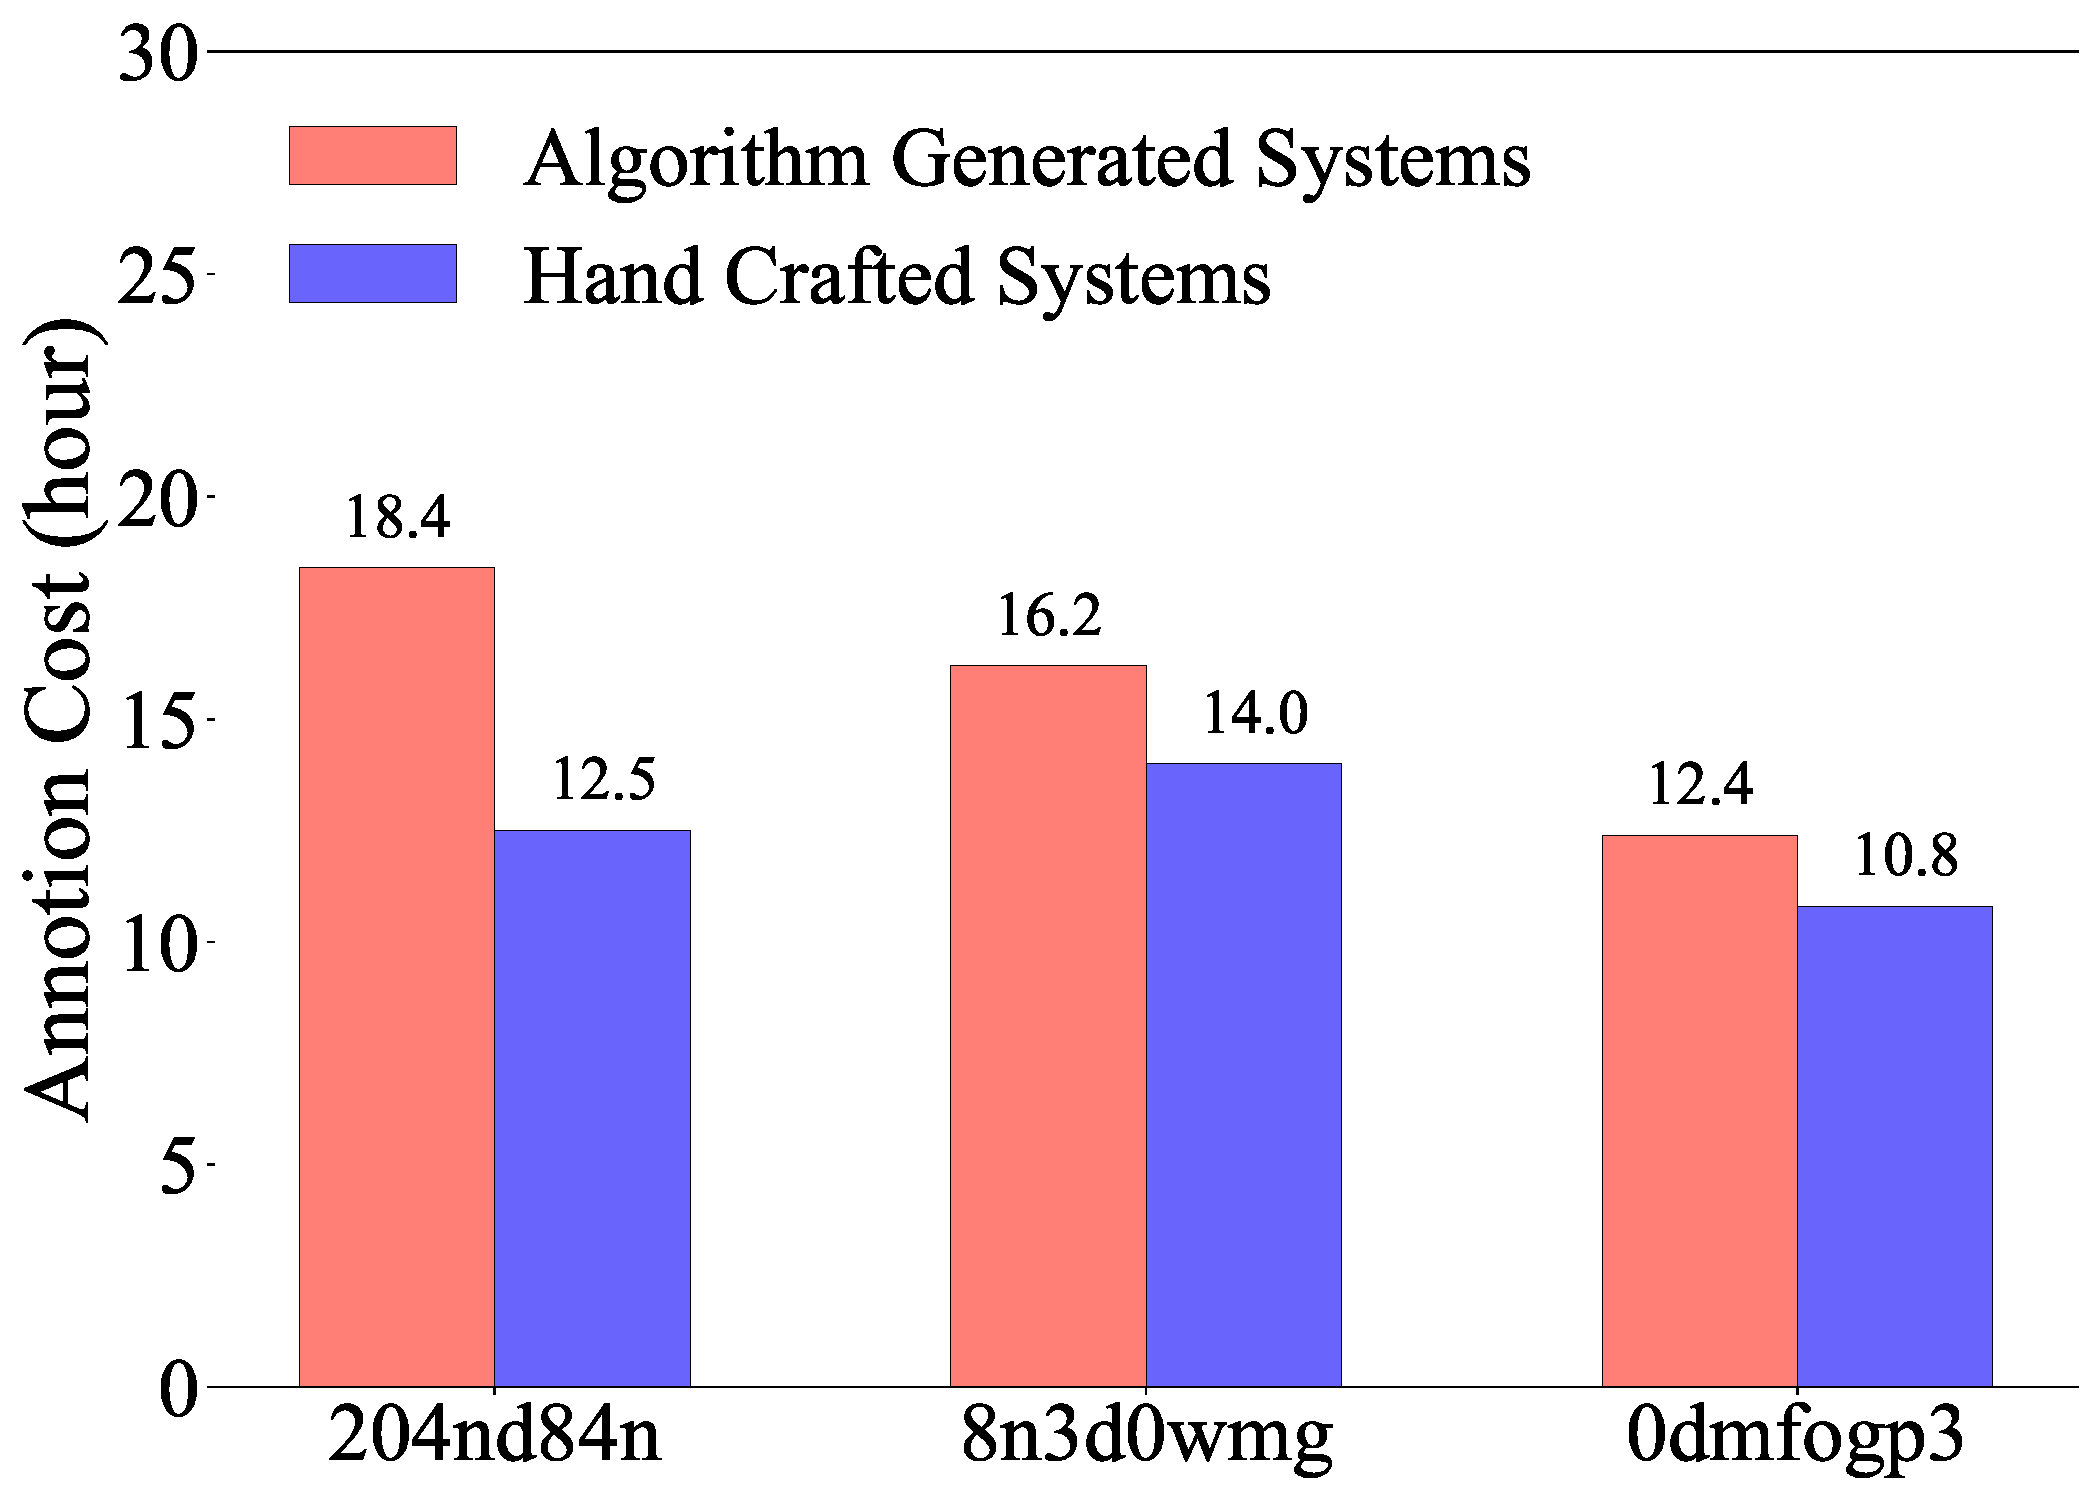
\includegraphics[width=0.3\textwidth]{fig/time_cost.pdf}
        \label{fig:labor_cost}
    }
    \subfigure[Uncertain annotation percentages.]{
        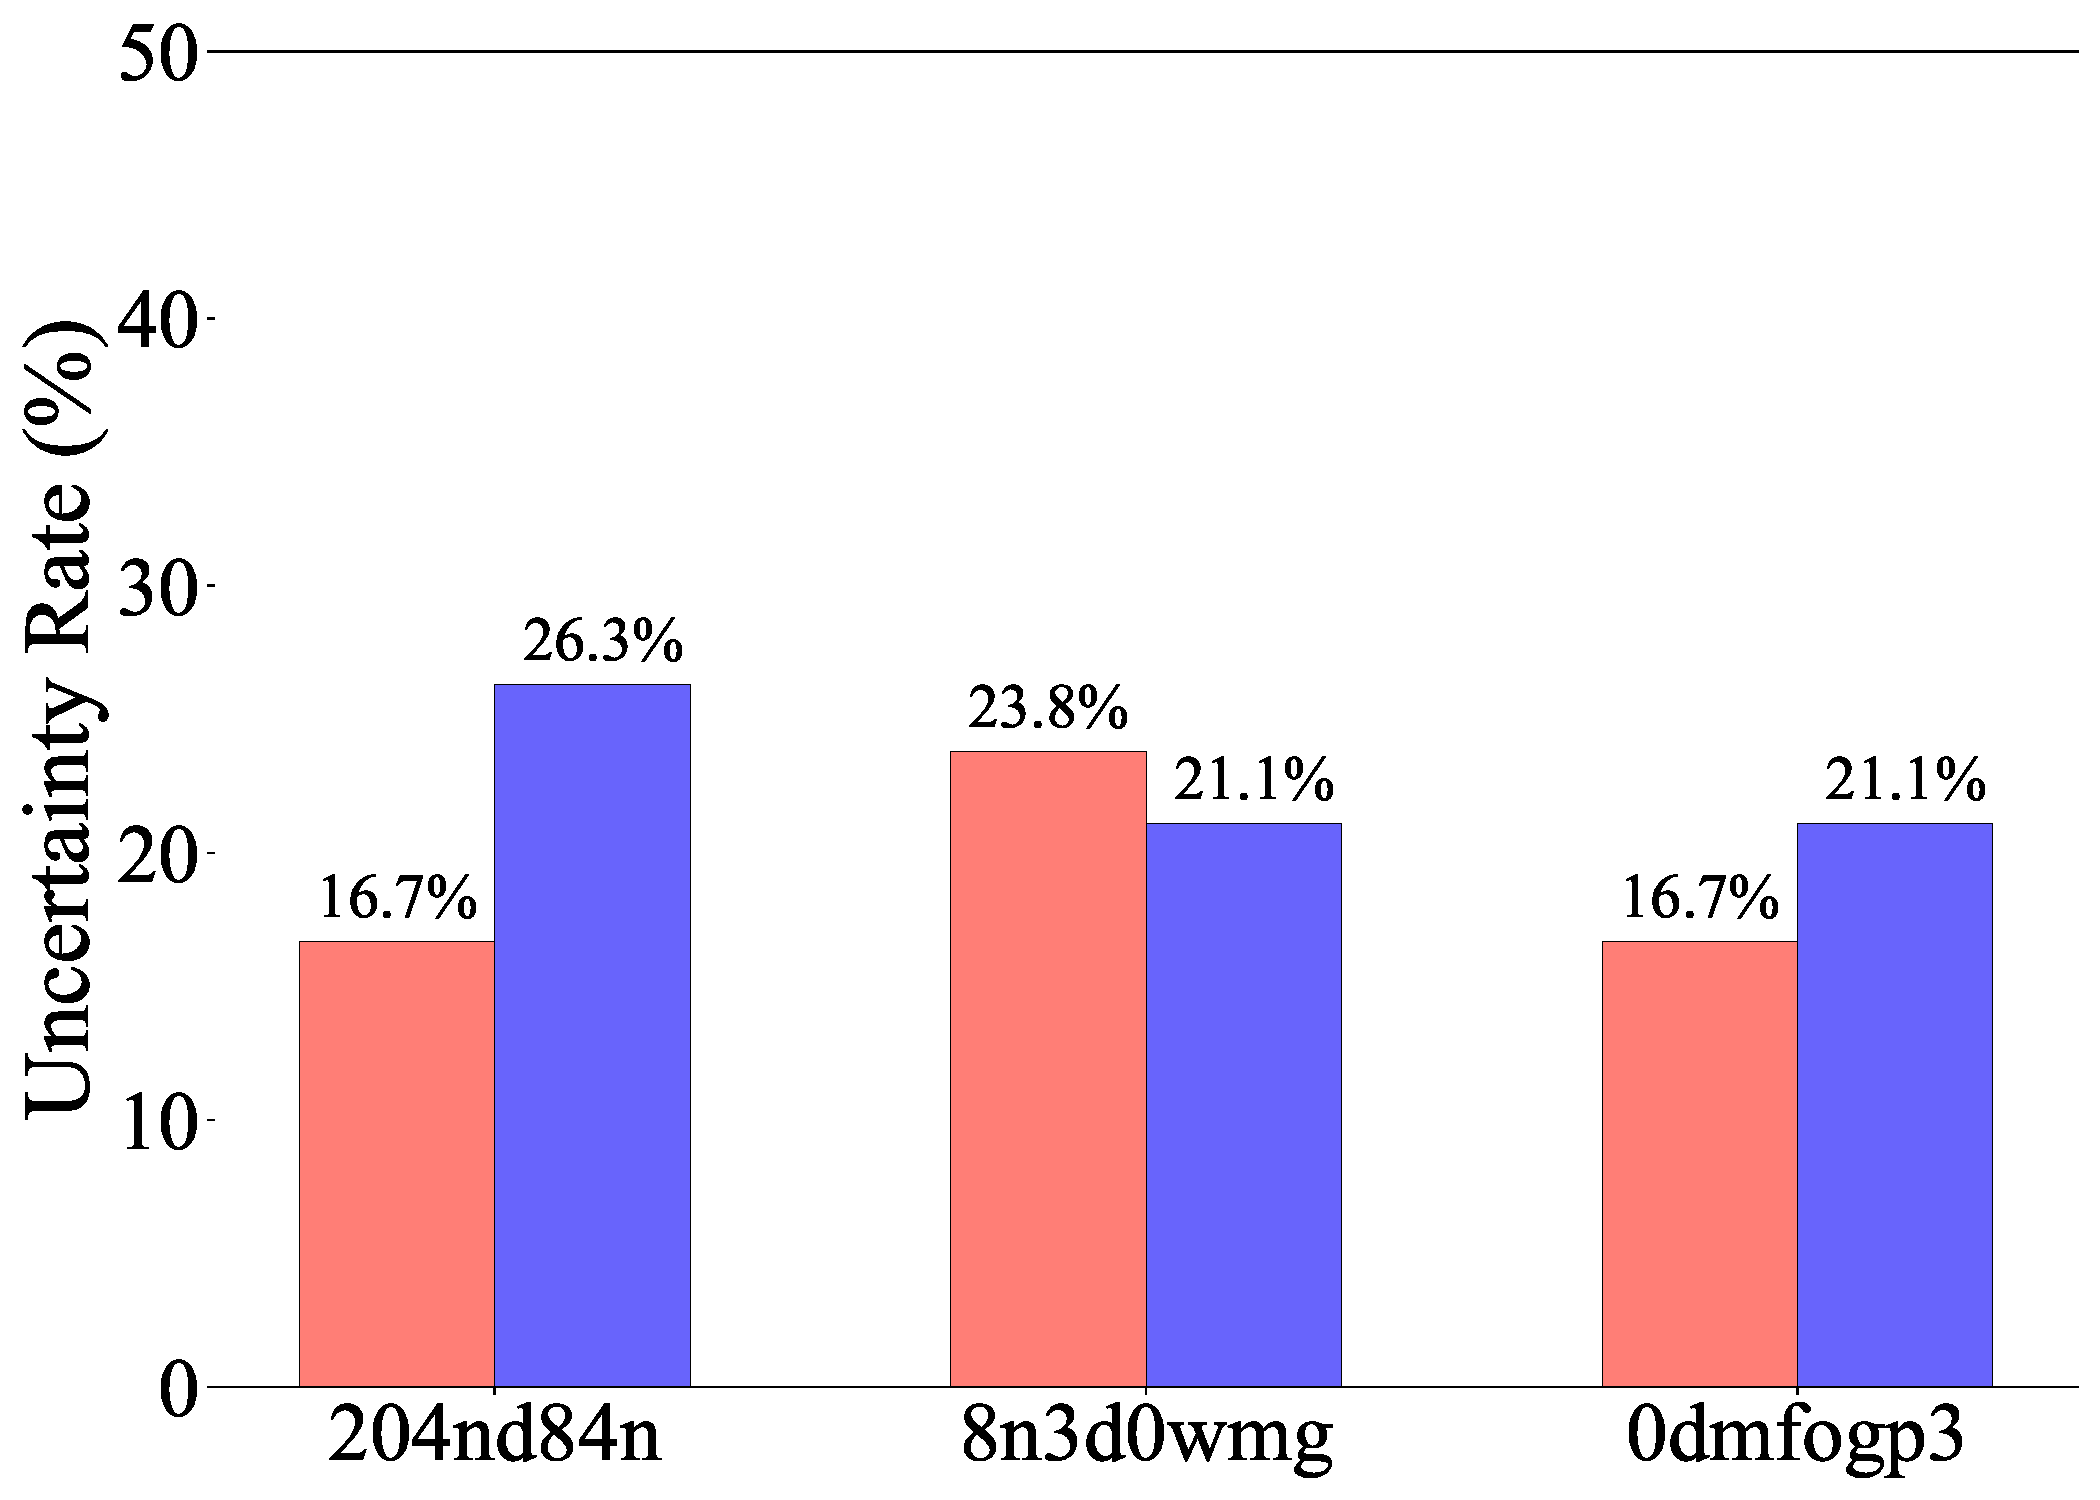
\includegraphics[width=0.31\textwidth]{fig/uncertain_rate.pdf}
        \label{fig:uncertain_rate}
    }
    \subfigure[Disagreement rates in voting.]{
        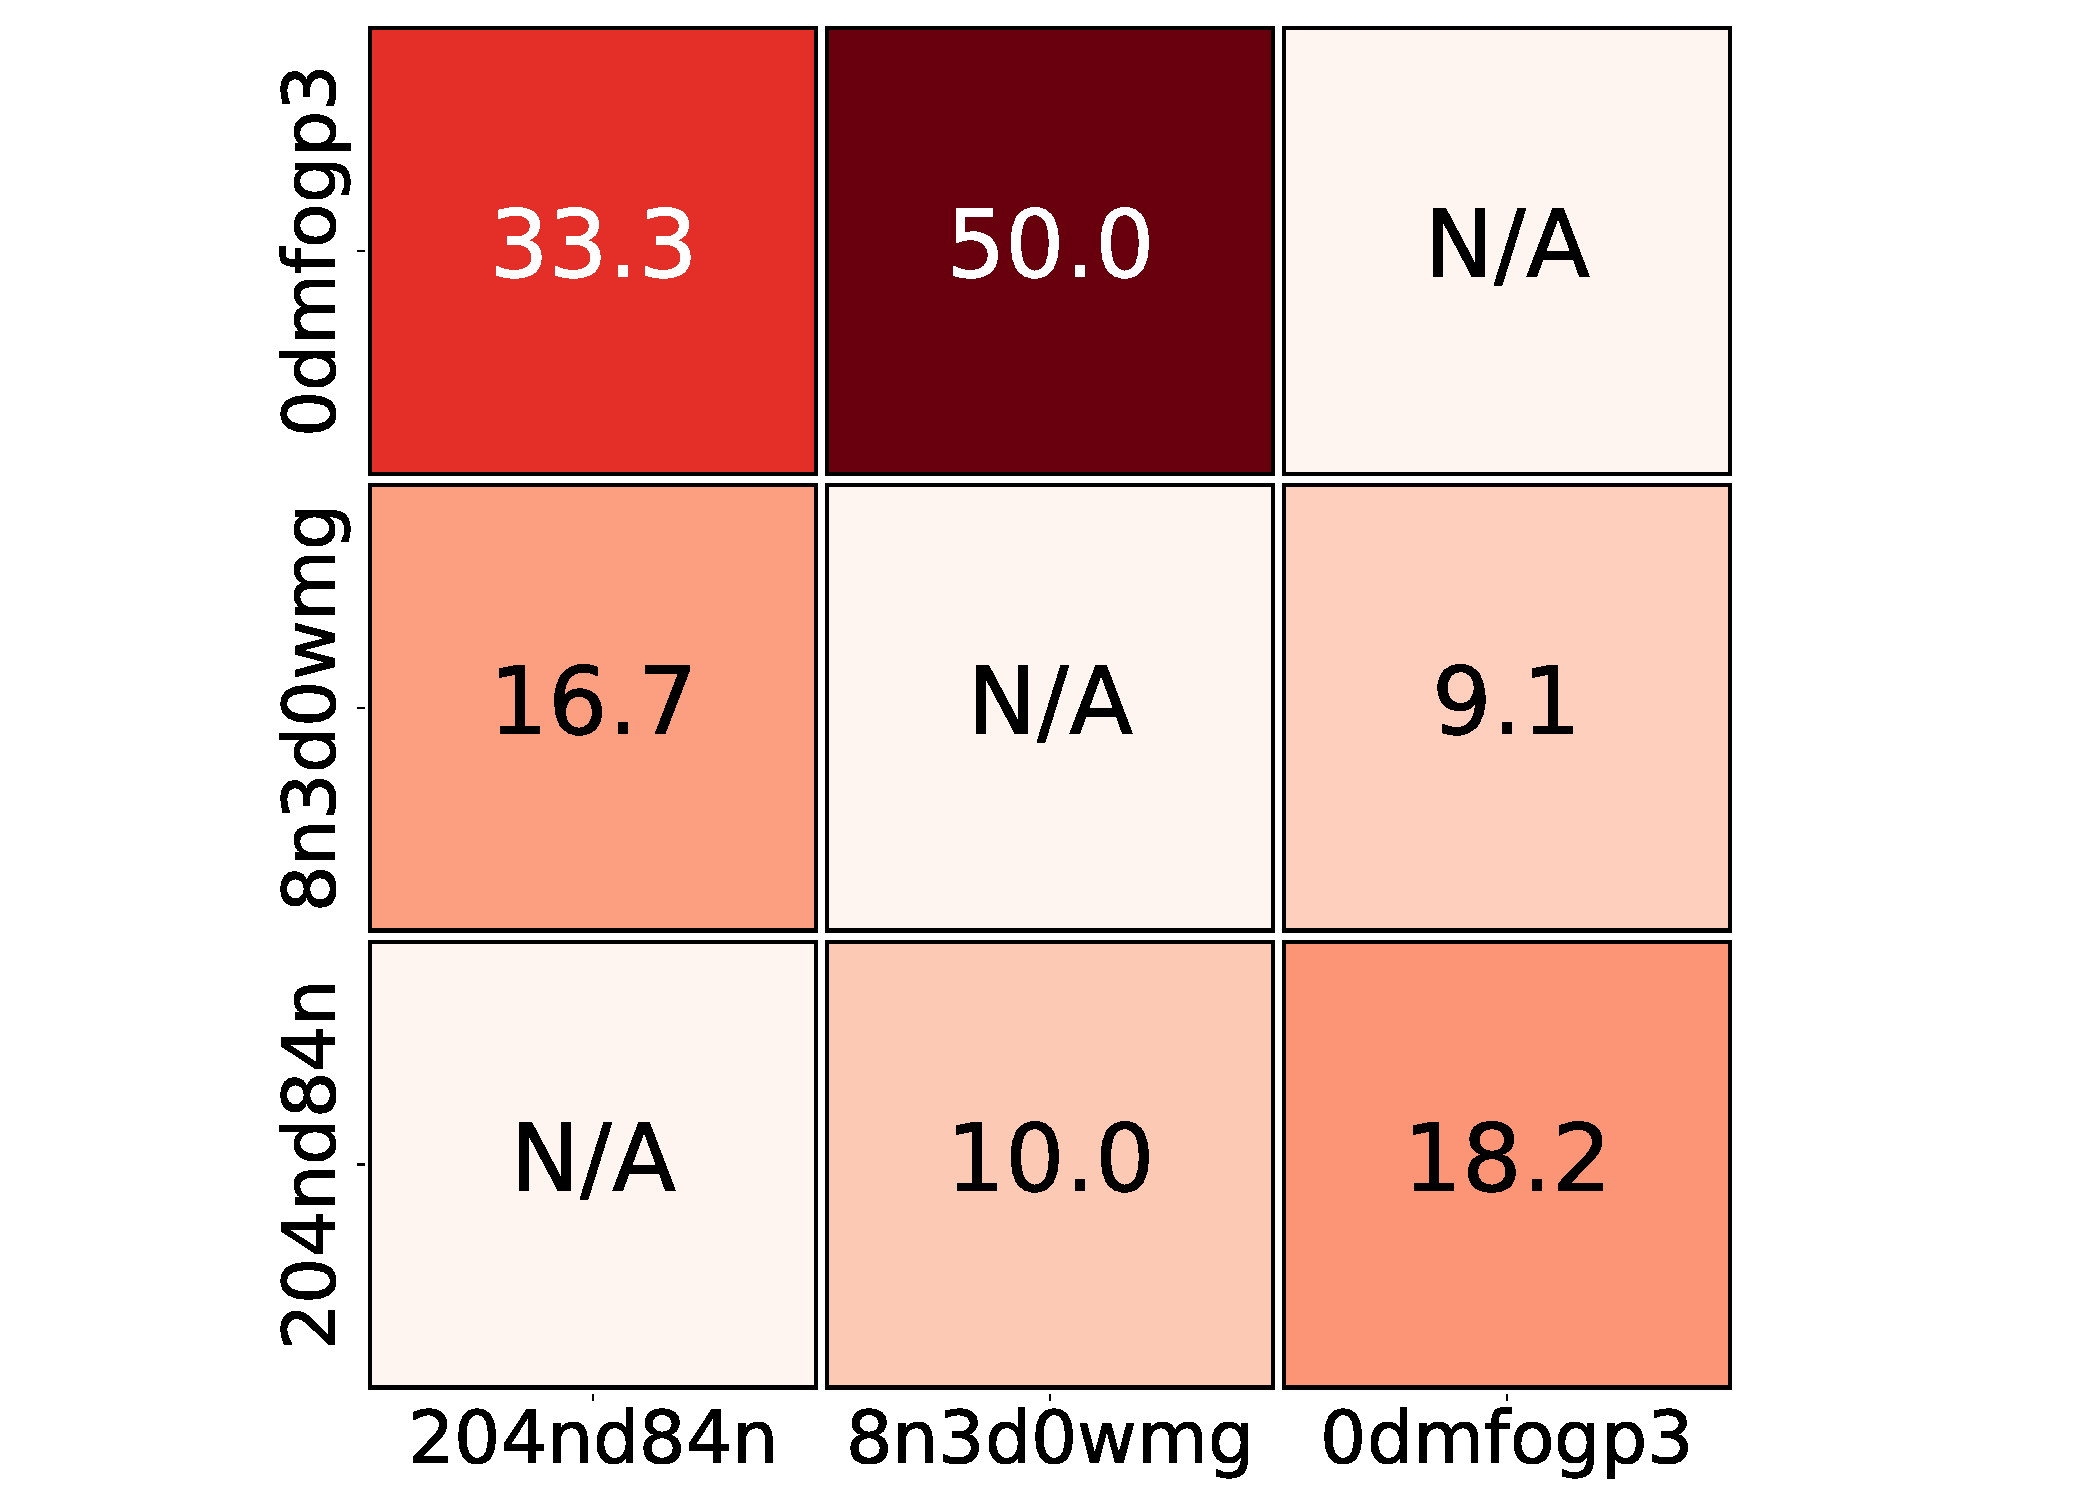
\includegraphics[width=0.3\textwidth]{fig/alg_dis.pdf}
        \label{fig:alg_dis}
    }
    \caption{Statistical analysis of the annotation process:
\textbf{(1)} Total labor cost for annotations in human hours.
\textbf{(2)} The proportion of uncertain annotations to total annotations during the second round.
\textbf{(3)} Initial disagreement rates between annotators (note that we make sure to reach a consensus through a careful discussion and voting process afterwards). These results highlight the challenges involved in performing manual failure attribution.}
\end{figure*}


\subsection{Agentic Systems Constructions} 

Who\&When includes two types of agentic systems: algorithm-generated agentic systems and one meticulously hand-crafted agentic systems, totaling 127 agentic systems equipped with diverse tools for evaluation. 

\paragraph{Algorithm-Generated Agentic Systems.}
To ensure an adequate number of agentic systems for the Who\&When datasets,  we first employ the CaptainAgent algorithm~\citep{song2024adaptive} from the AG2 library~\footnote{https://github.com/ag2ai/ag2} to automatically generate agentic systems for each data instance sourced from the validation sets of the GAIA~\citep{mialon2023gaia} and AssistantBench~\citep{yoran2024assistantbench} benchmarks. 
Specifically, it constructs a team of agents tailored to a given task, assigning appropriate agent names, prompts, and necessary tools. The system iteratively optimizes the agents' configuration until the task is successfully completed.
In the Who\&When, we select only the final multi-agent configurations, along with the corresponding execution history, as these represent the optimized solutions for each query. All agents within the constructed systems, as well as the CaptainAgent algorithm itself, are based on the \texttt{GPT-4o} on \texttt{2024-08-01-preview} version.
Additionally, since the primary objective of the Who\&When is to capture mistakes made by agents that lead to failures in solving real-world problems within agentic systems, we retain only those agentic systems that fail to successfully address the queries associated with each data instance from these benchmarks. 

\paragraph{Hand-Crafted Agentic Systems.}
In addition to algorithm-generated systems, Who\&When also includes a meticulously hand-crafted, mature multi-agent system, Magnetic-One~\citep{fourney2024magentic}, to ensure the representation of realistic and highly refined agentic systems. 
Magnetic-One is a generalist agentic system designed to handle a broad range of tasks. It comprises five carefully crafted agents, each specializing in distinct capabilities, such as operating a web browser or navigating local files. We evaluate Magnetic-One using the validation set from the AssistantBench~\citep{yoran2024assistantbench} benchmark, aggregating its failure logs for subsequent annotation.
We also test Magnetic-One on a randomly sampled subset of 30 instances from the GAIA~\citep{mialon2023gaia}, incorporating the corresponding execution failure logs into the dataset. We exclude the rest of the GAIA dataset due to the complexity of annotating the long context logs produced by Magentic-One. 

\subsection{Decisive Error Annotation}
After obtaining the failure logs of various agentic systems, we introduce an annotation procedure to identify the decisive error failure and decisive error step.
To ensure precise annotation, we conduct multiple rounds of annotation performed by three human experts in AI agent (whose identities are anonymized as 0dmfogp3, 8n3d0wmg, and 204nd84n).

\textbf{Round I:} In the first round, we distribute the failure logs from all agentic systems for each query equally among three experts. To ensure consistency, we provide the experts with a standardized annotation guideline as shown in Appendix~\ref{app:annotation}. Each expert is tasked with annotating three elements: the single erroneous agent primarily responsible for the task failure, the specific step at which the error occurred, and the reasoning behind the mistake in natural language. 
Additionally, each expert is required to categorize their annotations into two groups: those they are undoubtedly confident are correct and those they have any uncertainty about.
\textbf{Round II:} In the second round, people are instructed to make an agreement on all the uncertain annotations from Round II. For these uncertain annotations, we engage in a collaborative discussion to reach a consensus. We do not simply follow the principle of majority rule; instead, we aim to ensure that everyone is persuaded and that a consensus is ultimately reached.
\textbf{Round III:} In the final round, a cross-validation procedure is employed. Each expert is asked to go through another expert's annotations to assess the consistency of the annotation standards. If any discrepancies or issues with the annotations are identified, the experts engage in further discussion and, if necessary, re-annotate the data according to the established guidelines until a consensus is reached. Incorporating the viewpoints of multiple annotators and ensuring consensus among them, we aim to accurately reach the actual ground truth, as suggested by previous studies~\citep{clemen1989combining,zhuge2024agent}.

\subsection{Analysis}
\label{sec:dataset_analysis}

Annotating the decisive error agent and identifying the specific step of the error is challenging for both non-expert people and domain experts. The annotators must parse complex logs, follow the problem-solving logic of each agent, and assess whether each action is correct or if it misleads the entire problem-solving process.
For example, if an agent uses a web browser to gather essential information for problem-solving, annotators must check the browser history and visit each website to determine whether the failure is due to unavailable information on the website or because the agent failed to retrieve it.
As shown in Figure~\ref{fig:labor_cost}, three annotators spent 30.9, 30.2, and 23.2 human hours, respectively, to complete the annotations. This demonstrates that the annotation process is very time-consuming, leading us to consider doing research on automated failure attribution.

Additionally, in many data instances, it's not just one agent that makes mistakes, but several agents. People need to identify these mistakes and select the most severe ones, which can directly lead to problem-solving failures as formulated in Section~\ref{sec:problem_formulation}. Since the severity of mistakes may be subtle and even subjective at times, the process becomes even more difficult. As shown in Figure~\ref{fig:uncertain_rate}, we present the uncertain annotation percentages for three individuals. The uncertain percentages across different annotators range from 15\% to 30\%. We also visualize the disagreement rates between different individuals when voting on each other's uncertain data in Figure~\ref{fig:alg_dis}. We can see some disagreement remains before discussing to make the agreement, further highlighting the difficulties involved in the annotation process.

